\documentclass{article}
\usepackage{v-equation}
\usepackage{minted}
\usemintedstyle{staroffice}
\vgeometry
\begin{document}

\vspace*{\fill}
\begin{center}
\begin{tikzpicture}
[thick, scale=0.7, cap=round]
	\tzline(-7, 0)(7, 0)
	\tzellipse(0, 0)(0.4cm and 3cm)
	\tzline+[ultra thick] (-5, 0)(120:1)
	\tzanglemark(0, 0)(-5, 0)($(-5, 0)+(120:1)$){$\dfrac{2\pi}{3}$}[r]
	\tzline+[ultra thick] (6, 0)(-120:2)
	\tzanglemark(0, 0)(6, 0)($(6, 0)+(-120:2)$){$\alpha$}
	\tzline[|<->|]<0, -0.5>(-5, 0)(0, 0){$\dfrac{40}{3}$}[mb]
	\tzline+[|<->|]<-0.5, 0>($(6, 0)+(-120:2)$)(0, 2*sin{60}){$\dfrac{30\sqrt{3}}{13}$}[ml]
\end{tikzpicture}

\end{center}
\vspace*{\fill}
\pagebreak


\vspace*{\fill}
\inputminted[tabsize=4, breaklines, linenos=true, fontsize=\small]{tex}{tikz-2.tex}
\vspace*{\fill}

\pagebreak

\vspace*{\fill}
\begin{center}
\begin{tikzpicture}
	\foreach \a in {0, 8, ..., 352}{
		\tznode(\a:2){$+$}[scale=0.65]
		\tzdot[thin](\a:2)(6pt)
		\ifthenelse{\a=0}{}{
			\tzline[->]($(\a:2)!0.11cm!(0:2)$)($(\a:2)!4.5cm!(0:2)$)
		}	
	}
\end{tikzpicture}

\end{center}
\vspace*{\fill}
\pagebreak


\vspace*{\fill}
\inputminted[tabsize=4, breaklines, linenos=true, fontsize=\footnotesize]{tex}{tikz-3.tex}
\vspace*{\fill}

\pagebreak

\vspace*{\fill}
\begin{center}
\begin{tikzpicture}
[thick]
\def\A{16} %angle for element
\def\r{2} %radius
\def\dr{0.1} %delta r
\def\RO{\r+\dr} %radius outer
\def\RI{\r-\dr} %radius inner
\tzcoor(0:\RO)(O') %point at right end
\tzcoor*(0, 0)(O){$q_0$}[bl](5pt)
	\foreach \a in {0, 8, ..., 352}{
		\tznode(\a:\r){$+$}[scale=0.65]
		\draw[thin](\a:\r) circle [radius=\dr];
	}
	\tzlines(O)(\A:\RO)(O)(-\A:\RO);
	\tzarc(O)(-\A:\A:\RO)
	\tzarc(O)(-\A:\A:\RI)
	\tzline[->](\A:\RO)($(\A:\RO)!2cm!(1.01*\A:\RO)$){$\Delta T$}[a]
	\tzline[->](-\A:\RO)($(-\A:\RO)!2cm!(-1.01*\A:\RO)$){$\Delta T$}[b]
	\tzline+[->](O')(2, 0){$\Delta F_e$}[r]
	\tzanglemark'(-\A:\r)(O)(\A:\r){$\d{\theta}$}(15pt)
	\tzline[<->, thick]($(O')+(0,2.5)$)($(O')+(0,-2.5)$)
	\tzarc[thick](O')(90:90+0.7*\A:1){$\d{\theta}/2$}[a=2mm, r=1mm]
	\tzarc[thick](O')(270-0.7*\A:270:1)
\end{tikzpicture}

\end{center}
\vspace*{\fill}
\pagebreak


\vspace*{\fill}
\inputminted[tabsize=4, breaklines, linenos=true, fontsize=\small]{tex}{tikz-4.tex}
\vspace*{\fill}

\pagebreak

\vspace*{\fill}
\begin{center}
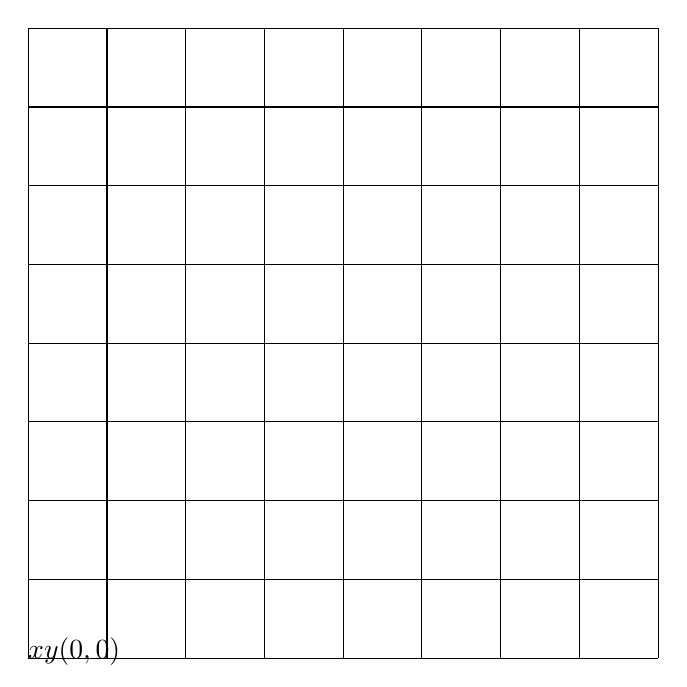
\begin{tikzpicture}
\draw (0, 0) grid (8, 8);
\tzaxes(0, 0)(8.5,8.5){$x$}{$y$}
\tzcoor*(0, 0)(O){$(0, 0)$}[bl]

	\tzline+[->, red](O)(4,0)
	\tzline+[->, red](4, 0)(0,5)
	\tzline[->, green](O)(4, 5)


\end{tikzpicture}

\end{center}
\vspace*{\fill}
\pagebreak


\vspace*{\fill}
\inputminted[tabsize=4, breaklines, linenos=true, fontsize=\small]{tex}{tikz-5.tex}
\vspace*{\fill}

\end{document}
